\documentclass[12pt,a4paper]{article}

% ============================================================================
% PAQUETES Y CONFIGURACIONES
% ============================================================================
\usepackage[utf8]{inputenc}
\usepackage[T1]{fontenc}
\usepackage[spanish,es-tabla]{babel}
\usepackage{geometry}
\geometry{top=2.5cm, bottom=2.5cm, left=2.5cm, right=2.5cm}

\usepackage{graphicx}
\usepackage{xcolor}
\usepackage{fancyhdr}
\usepackage{listings}
\usepackage{hyperref}
\usepackage{booktabs}
\usepackage{amsmath}
\usepackage{tabularx}
\usepackage{float}
\usepackage{enumitem}

\hypersetup{
    colorlinks=true,
    linkcolor=black,
    urlcolor=blue!80!black,
    citecolor=blue!80!black
}

% Paleta institucional
\definecolor{unsaacred}{RGB}{122, 31, 43}
\definecolor{unsaacgold}{RGB}{201, 151, 31}
\definecolor{cafedark}{RGB}{62, 39, 35}
\definecolor{codegray}{rgb}{0.5,0.5,0.5}
\definecolor{backcolour}{rgb}{0.97,0.98,0.99}
\definecolor{keywordblue}{rgb}{0.0,0.2,0.7}
\definecolor{stringgreen}{rgb}{0.1,0.5,0.2}

\lstdefinelanguage{Dart}{
    keywords={abstract, as, assert, async, await, break, case, catch, class,
    const, continue, default, do, dynamic, else, enum, export, extends,
    false, final, finally, for, Function, get, if, in, is, late, new, null,
    rethrow, return, super, switch, this, throw, true, try, var, void, while,
    required, set, static, factory, override},
    morekeywords=[2]{int, double, String, bool, List, Map, Set, num, DateTime,
    Widget, BuildContext, StatelessWidget, StatefulWidget, State, Key, Color,
    EdgeInsets, EdgeInsetsDirectional, BoxDecoration, BorderRadius, BoxShadow,
    Offset, Radius, Border, TextStyle, FontWeight, FontStyle, MainAxisSize,
    MainAxisAlignment, CrossAxisAlignment, TextAlign, BoxShape, LayoutBuilder,
    BoxConstraints, GridView, ListView, ClipRRect, Stack, Positioned, Wrap, FilterChip},
    keywordstyle=\color{keywordblue}\bfseries,
    keywordstyle=[2]\color{unsaacred}\bfseries,
    identifierstyle=\color{black},
    sensitive=true,
    comment=[l]{//},
    commentstyle=\color{codegray}\itshape,
    stringstyle=\color{stringgreen},
    morestring=[b]',
    morestring=[b]"
}

\lstset{
    language=Dart,
    backgroundcolor=\color{backcolour},
    basicstyle=\ttfamily\footnotesize,
    breaklines=true,
    breakatwhitespace=false,
    frame=single,
    rulecolor=\color{gray!30},
    numbers=left,
    numberstyle=\tiny\color{codegray},
    numbersep=6pt,
    captionpos=b,
    showspaces=false,
    showstringspaces=false,
    tabsize=2,
    literate=
      {á}{{\'a}}1 {é}{{\'e}}1 {í}{{\'i}}1 {ó}{{\'o}}1 {ú}{{\'u}}1
      {Á}{{\'A}}1 {É}{{\'E}}1 {Í}{{\'I}}1 {Ó}{{\'O}}1 {Ú}{{\'U}}1
      {ñ}{{\~n}}1 {Ñ}{{\~N}}1 {¿}{{?`}}1 {¡}{{!`}}1
}

\pagestyle{fancy}
\fancyhf{}
\fancyhead[L]{\small UNSAAC — EPIIS (IF616AIN)}
\fancyhead[R]{\small Proyecto Integrador 2: Catálogo de Emprendimiento (Grupo 2)}
\fancyfoot[C]{\thepage}
\renewcommand{\headrulewidth}{0.4pt}

\begin{document}

% ============================================================================
% PORTADA INSTITUCIONAL
% ============================================================================
\begin{titlepage}
    \centering
    \vspace*{0.2cm}
    {\Large \textbf{UNIVERSIDAD NACIONAL DE SAN ANTONIO ABAD DEL CUSCO}}\\[0.2cm]
    {\large \textbf{FACULTAD DE INGENIERÍA ELÉCTRICA, ELECTRÓNICA, INFORMÁTICA Y MECÁNICA}}\\[0.2cm]
    {\normalsize \textbf{ESCUELA PROFESIONAL DE INGENIERÍA INFORMÁTICA Y DE SISTEMAS}}\\[0.6cm]

    
\includegraphics[width=3.6cm]{imagenes/unsaac_logo.png}\\[0.5cm]

    \rule{\linewidth}{0.8pt}\\[0.3cm]
    {\Large \textbf{PROYECTO INTEGRADOR N$^\circ$ 2 — TRABAJO EN EQUIPO}}\\[0.2cm]
    {\large \textbf{Catálogo de Productos de un Emprendimiento Local Cusqueño}}\\[0.2cm]
    {\normalsize \textit{«Aroma Sagrado»: Café Especial y Cacao Chuncho de La Convención}}\\[0.2cm]
    {\small Unidad Didáctica I: Fundamentos de Dart, UI Declarativa y Experiencia de Usuario}\\[0.2cm]
    \rule{\linewidth}{0.8pt}\\[0.5cm]

    \begin{flushleft}
        \textbf{Asignatura:} Desarrollo de Software II (IF616AIN) — Semestre Académico 2026-II\\
        \textbf{Docente:} Mtro. Ing. Yover Collantes Valer\\
        \textbf{Horario / Aula:} Lunes y Miércoles 16:00 - 18:00 (Aula IN304)\\[0.2cm]
        \textbf{Equipo de Trabajo:} \textbf{GRUPO 2}\\[0.15cm]
        \textbf{Integrantes:}\\
        • Edmil Jampier Saire Bustamante \hfill (Código: 174449)\\
        • Alain Armando Condori Contreras\\
        • Axel Aranibar Rojas\\[0.2cm]
        \textbf{Fecha de Entrega:} Cusco, 07 de Octubre de 2026
    \end{flushleft}

    \vfill
    {\small Cusco, Perú\\2026}
\end{titlepage}

\newpage

% ============================================================================
% 1. INTRODUCCIÓN Y OBJETIVOS
% ============================================================================
\section{Introducción y Objetivos}

El presente informe documenta el desarrollo y maquetación del \textbf{Proyecto Integrador 2: Catálogo de Productos de un Emprendimiento Local}, correspondiente a la culminación de la Primera Unidad Didáctica de la asignatura \textit{Desarrollo de Software II (IF616AIN)}.

El proyecto asignado al \textbf{Grupo 2} consistió en la concepción y materialización de la aplicación móvil para el emprendimiento cusqueño \textbf{«Aroma Sagrado»}, dedicado a la comercialización de cafés de especialidad (variedades Geisha, Bourbon y Typica) y derivados de cacao fino de aroma (Chuncho nativo) provenientes de los valles cafetaleros de Santa Teresa, Echarati y Ocobamba en la provincia de La Convención, Cusco.

\subsection{Objetivos Técnicos}
\begin{enumerate}[leftmargin=*]
    \item \textbf{Dominio del Modelo de Restricciones:} Implementar una composición visual sin errores de desbordamiento (\textit{RenderFlex overflowed}) ni restricciones infinitas (\textit{unbounded}), respetando rigurosamente el axioma fundamental de Flutter: \textit{«Constraints go down, sizes go up, parent sets position»}.
    \item \textbf{Composición Integral de Widgets:} Utilizar de forma armónica los widgets de layout y contenido estudiados a lo largo de las sesiones 4 a 9 (\texttt{Container}, \texttt{Row}, \texttt{Column}, \texttt{Expanded}, \texttt{Stack}, \texttt{Positioned}, \texttt{Wrap}, \texttt{GridView}, \texttt{ListView} y \texttt{LayoutBuilder}).
    \item \textbf{Diseño Adaptativo y Responsivo:} Garantizar que la cuadrícula del catálogo reorganice automáticamente su distribución visual según el ancho disponible del dispositivo (2 columnas en móviles, 3 columnas en tabletas y 4 columnas en pantallas anchas/escritorio).
    \item \textbf{Estándar de Calidad UI/UX:} Diseñar una interfaz pulcra, institucional y comercialmente viable, con jerarquía tipográfica de tres niveles, contraste verificado y zonas táctiles accesibles ($\ge 48 \times 48\text{ dp}$).
\end{enumerate}

% ============================================================================
% 2. ARQUITECTURA DE WIDGETS Y ESTRUCTURA DEL CÓDIGO
% ============================================================================
\section{Arquitectura de Widgets y Estructura del Código}

La aplicación fue desarrollada como un proyecto Flutter formal e independiente bajo el principio de modularidad y responsabilidad única (DRY).

\subsection{Estructura de Directorios del Proyecto}
\begin{lstlisting}[language=bash]
app_catalogo_grupo2/
|-- lib/
|   |-- data/
|   |   |-- catalogo_data.dart        // Dataset con 8 productos y 3 recomendaciones
|   |-- models/
|   |   |-- producto.dart             // Entidad inmutable con tipado estricto
|   |-- screens/
|   |   |-- catalogo_screen.dart      // Pantalla principal con LayoutBuilder
|   |-- widgets/
|   |   |-- banner_promocional.dart   // Banner con Stack, degradado y badge
|   |   |-- cabecera_institucional.dart// Ficha academica oficial del Grupo 2
|   |   |-- filtro_categorias.dart    // Fila de filtros con Wrap y FilterChip
|   |   |-- panel_emprendimiento_info.dart // Compromiso de comercio justo
|   |   |-- seccion_interesar.dart    // Carrusel horizontal con ListView
|   |   |-- tarjeta_producto.dart     // Card con imagen, Stack y precios
|   |-- main.dart                     // Configuracion de MaterialApp y tema
|-- test/
|   |-- screenshot_generator_test.dart// Generador automatizado de capturas HD
|   |-- widget_test.dart              // Pruebas de inicializacion de UI
|-- pubspec.yaml                      // Metadatos y dependencias
\end{lstlisting}

\subsection{Blueprint del Árbol de Widgets Principal}
\begin{lstlisting}[language=bash]
MaterialApp (ThemeData institucional granate y dorado)
  |-- Scaffold
        |-- AppBar (Aroma Sagrado Cusco + Acciones de busqueda y carrito)
        |-- body: SingleChildScrollView
        |     |-- Column (crossAxisAlignment: stretch)
        |           |-- CabeceraInstitucional (UNSAAC + Grupo 2)
        |           |-- BannerPromocional (StackFit.expand + LinearGradient)
        |           |-- _seccion('Explorar por Categoria')
        |           |-- FiltroCategorias (Wrap + FilterChip)
        |           |-- _seccion('Catalogo de Productos de Temporada')
        |           |-- LayoutBuilder (Calculo dinamico de columnas)
        |           |     |-- GridView.builder (crossAxisCount: 2 | 3 | 4)
        |           |           |-- TarjetaProducto (Stack + ClipRRect + Precios)
        |           |-- _seccion('Tambien te puede interesar')
        |           |-- SeccionInteresar (ListView horizontal)
        |           |-- _seccion('Nuestra Historia y Origen')
        |           |-- PanelEmprendimientoInfo (Sellos de Comercio Justo)
        |-- bottomNavigationBar: BottomNavigationBar (4 items estaticos)
\end{lstlisting}

% ============================================================================
% 3. IMPLEMENTACIÓN DE REQUERIMIENTOS Y DECISIONES DE DISEÑO
% ============================================================================
\section{Implementación de Requerimientos y Decisiones Técnicas}

A continuación se detalla cómo el Grupo 2 dio cumplimiento exacto a cada uno de los requerimientos obligatorios especificados en el capítulo 12 del documento curricular de la Sesión 6:

\subsection{Requerimiento 1: Banner Superior con \texttt{Stack} y \texttt{StackFit.expand}}
Se construyó un contenedor de $200\text{ dp}$ de altura envuelto en \texttt{ClipRRect(borderRadius: BorderRadius.circular(16))}. En su interior, un \texttt{Stack} con \texttt{fit: StackFit.expand} superpone:
\begin{enumerate}
    \item La fotografía de fondo del cafetal cusqueño con \texttt{BoxFit.cover}.
    \item Un degradado vertical oscuro (\texttt{LinearGradient}) mediante \texttt{Positioned.fill} para otorgar contraste al texto blanco sobre la imagen.
    \item Una insignia superior de denominación de origen (\textit{«ORIGEN CUSCO · 100\% ORGÁNICO»}) con \texttt{Positioned(top: 14, left: 14)}.
    \item Los textos promocionales anclados en la base mediante \texttt{Positioned(bottom: 14, left: 16, right: 16)}.
\end{enumerate}

\subsection{Requerimiento 2: Fila de Filtros de Categoría con \texttt{Wrap}}
En lugar de utilizar una \texttt{Row} rígida que desbordaría en pantallas angostas, se implementó el widget \texttt{Wrap} con \texttt{spacing: 8.0} y \texttt{runSpacing: 8.0}. Esto permite que las 6 categorías (*Todos, Café Especial, Cacao Chuncho, Miel Orgánica, Métodos \& Prensa, Packs Regalo*) se acomoden automáticamente en múltiples líneas de manera fluida.

\subsection{Requerimientos 3 y 4: Rejilla de 8 Productos y Etiquetas de Oferta con \texttt{Stack}}
La rejilla principal renderiza 8 productos de alta calidad mediante \texttt{GridView.builder}. Cada tarjeta (\texttt{TarjetaProducto}) integra:
\begin{itemize}
    \item Imagen del producto dentro de \texttt{ClipRRect(borderRadius: BorderRadius.vertical(top: Radius.circular(16)))}.
    \item Insignia de descuento (\texttt{-20\%}, \texttt{-18\%}, \texttt{-15\%}) o novedad (\texttt{NUEVO}) superpuesta en la esquina superior izquierda mediante \texttt{Stack} y \texttt{Positioned(top: 8, left: 8)}.
    \item Botón táctil de favoritos en la esquina superior derecha con \texttt{Positioned(top: 4, right: 4)} y área táctil accesible de $40 \times 40\text{ dp}$.
    \item Nombre del producto con \texttt{maxLines: 2} y \texttt{overflow: TextOverflow.ellipsis}.
    \item Fila de calificación con estrella dorada \texttt{Icon(Icons.star, color: Color(0xFFFFA000))} y número de reseñas.
    \item Precio actual en tipografía destacada (\texttt{Color(0xFF7A1F2B)}) y precio anterior tachado en gris (\texttt{TextDecoration.lineThrough}) cuando existe descuento activo.
    \item Botón de compra rápido con ícono \texttt{Icons.add\_shopping\_cart}.
\end{itemize}

\subsection{Requerimiento 5: Sección «También te puede interesar» con \texttt{ListView} Horizontal}
Se implementó un carrusel de recomendaciones horizontales mediante \texttt{ListView.builder(scrollDirection: Axis.horizontal)} alojado en un contenedor de $180\text{ dp}$ de altura. Cada tarjeta compacta ($260\text{ dp}$ de ancho) organiza la imagen y los datos en una \texttt{Row} equilibrada.

\subsection{Requerimiento 6: Encabezado Reutilizable (\texttt{Widget \_seccion})}
Siguiendo las buenas prácticas DRY de Flutter, los encabezados de sección se centralizaron en la función privada \texttt{Widget \_seccion(String titulo)}, garantizando coherencia visual en tipografía, colores (\texttt{Color(0xFF3E2723)}) y espaciados de margen.

% ============================================================================
% 4. ADAPTABILIDAD Y COMPORTAMIENTO RESPONSIVO
% ============================================================================
\section{Adaptabilidad y Comportamiento Responsivo}

En estricto cumplimiento de la consigna adaptativa exigida, la rejilla principal de productos utiliza \texttt{LayoutBuilder} para calcular en tiempo de ejecución el número óptimo de columnas (\texttt{crossAxisCount}) en función del ancho disponible:

\begin{equation}
\text{crossAxisCount}(\text{maxWidth}) = 
\begin{cases} 
2 & \text{si } \text{maxWidth} < 600\text{ pt (Dispositivos Móviles en vertical)} \\
3 & \text{si } 600 \le \text{maxWidth} < 840\text{ pt (Tabletas y móviles apaisados)} \\
4 & \text{si } \text{maxWidth} \ge 840\text{ pt (Monitores de escritorio y pantallas anchas)}
\end{cases}
\end{equation}

\begin{table}[H]
\centering
\begin{tabularx}{\textwidth}{@{}lcccc@{}}
\toprule
\textbf{Categoría de Pantalla} & \textbf{Rango de Ancho} & \textbf{Columnas} & \textbf{Relación Aspecto} & \textbf{Experiencia de Usuario} \\ \midrule
\textbf{Compacta (Móvil)} & $< 600\text{ pt}$ & 2 & 0.68 & Tarjetas cómodas para interacción táctil \\
\textbf{Media (Tableta)} & $600 - 839\text{ pt}$ & 3 & 0.72 & Aprovechamiento horizontal sin vacíos \\
\textbf{Expandida (Escritorio)} & $\ge 840\text{ pt}$ & 4 & 0.75 & Visualización tipo vitrina panorámica \\ \bottomrule
\end{tabularx}
\caption{Matriz de puntos de quiebre y adaptación del catálogo de productos.}
\end{table}

% ============================================================================
% 5. RESULTADOS Y EVIDENCIAS VISUALES
% ============================================================================
\section{Resultados y Evidencias Visuales}

Las siguientes figuras presentan las capturas de pantalla reales capturadas directamente desde el motor de renderizado de Flutter en alta resolución, certificando la fidelidad visual, la ausencia de desbordamientos y el comportamiento adaptativo de la interfaz.

\begin{figure}[H]
    \centering
    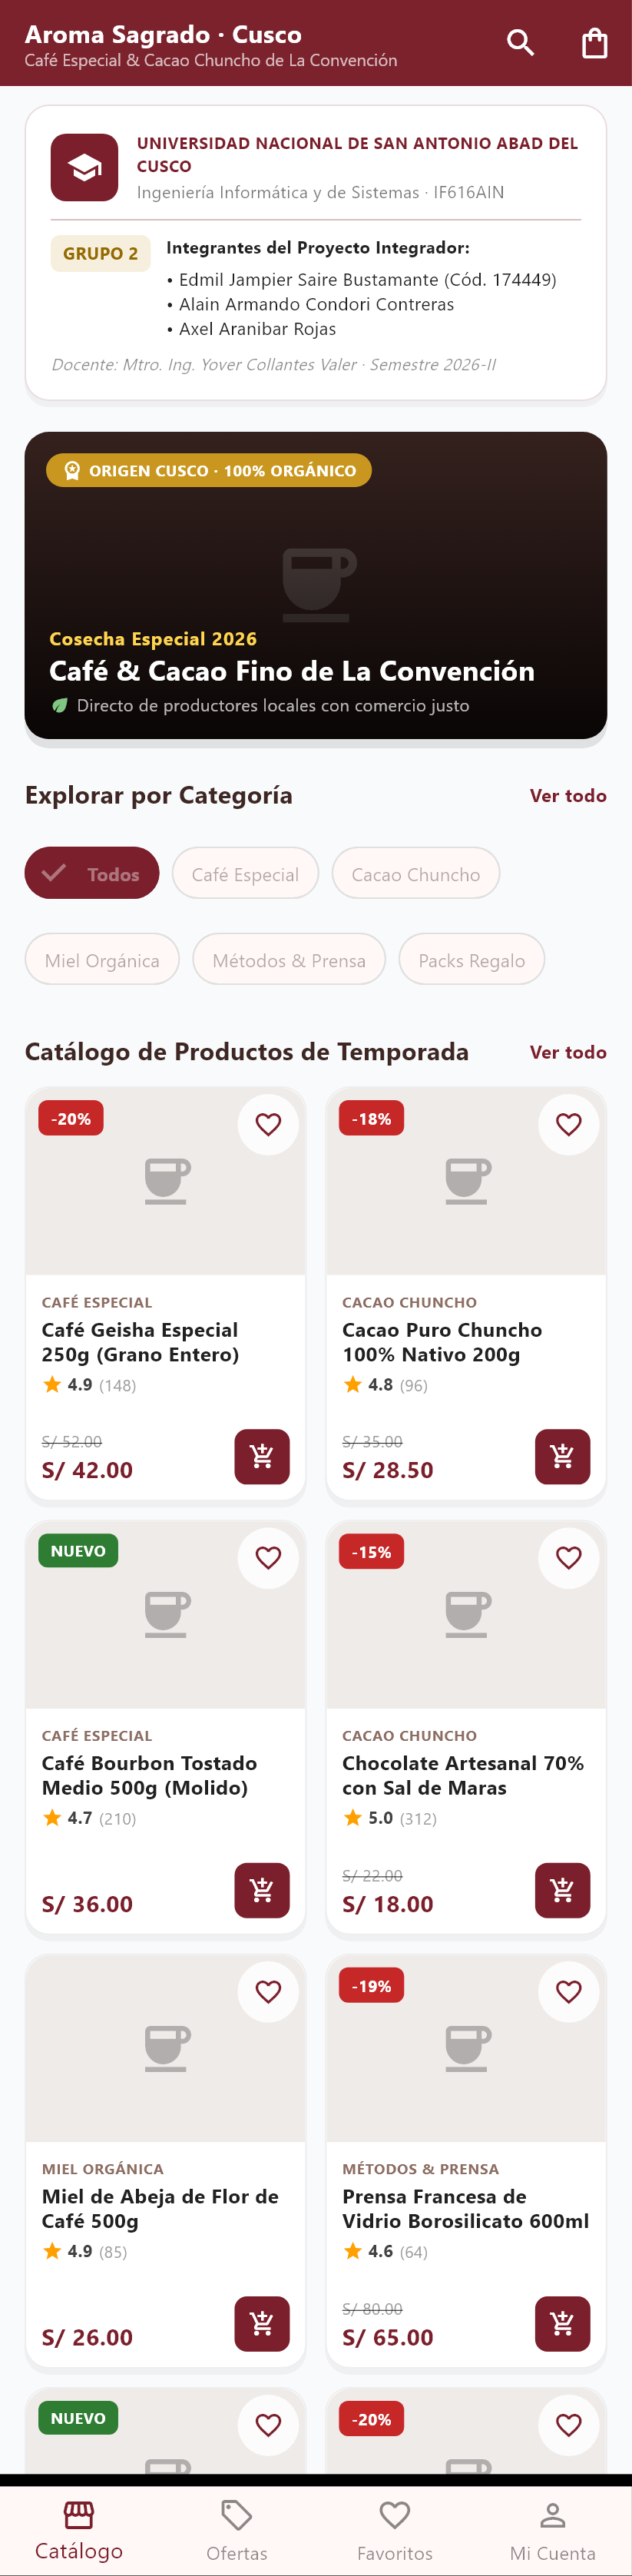
\includegraphics[width=0.48\textwidth]{imagenes/captura_catalogo_movil.png}
    \caption{Vista del Catálogo en Dispositivo Móvil ($< 600\text{ pt}$, 2 columnas en GridView).}
\end{figure}

\begin{figure}[H]
    \centering
    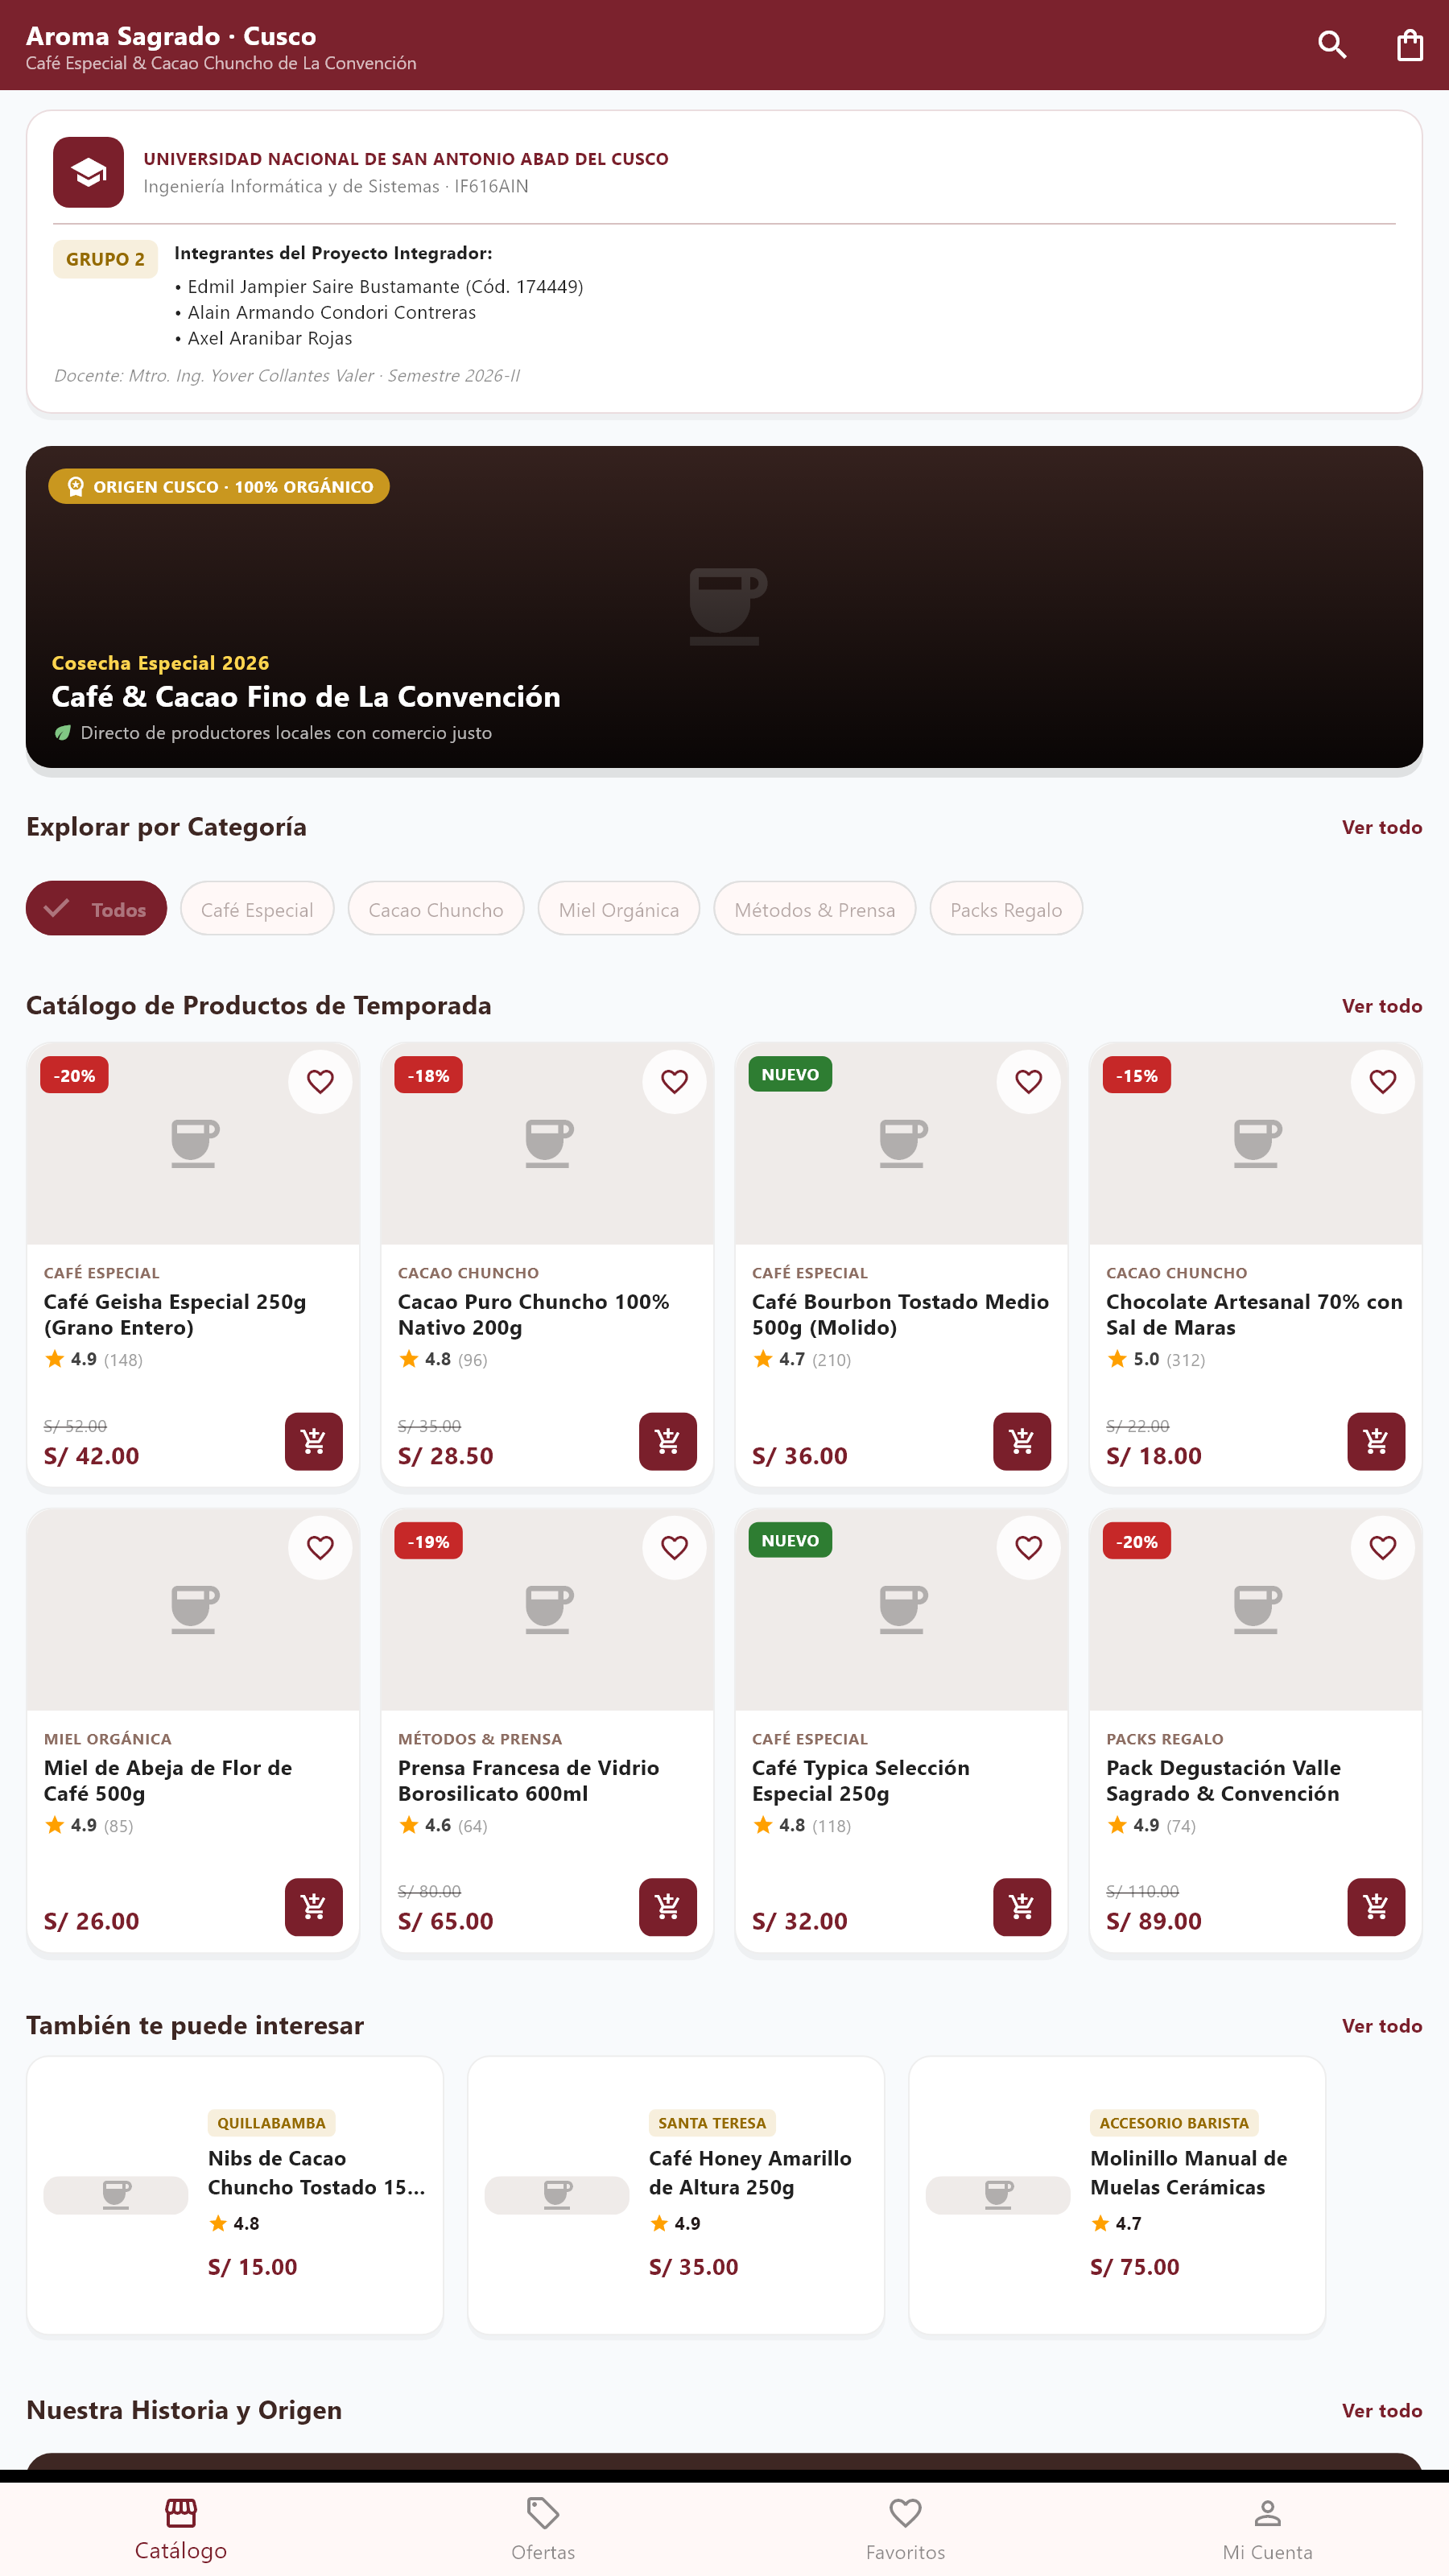
\includegraphics[width=0.95\textwidth]{imagenes/captura_catalogo_tableta.png}
    \caption{Vista del Catálogo en Tableta / Pantalla Ancha ($\ge 840\text{ pt}$, 4 columnas en GridView con carrusel inferior).}
\end{figure}

% ============================================================================
% 6. DIFICULTADES ENCONTRADAS Y SOLUCIONES
% ============================================================================
\section{Dificultades Encontradas y Soluciones}

\begin{enumerate}[leftmargin=*]
    \item \textbf{Dificultad: Anidamiento de \texttt{GridView} dentro de \texttt{SingleChildScrollView}}.\\
    \textbf{Causa:} \texttt{SingleChildScrollView} proporciona altura infinita (\textit{unbounded}) a su hijo, lo que entra en conflicto con el comportamiento de scroll propio de \texttt{GridView}.\\
    \textbf{Solución:} Se configuró \texttt{shrinkWrap: true} y \texttt{physics: const NeverScrollableScrollPhysics()} en el \texttt{GridView}, permitiendo que delegue su cálculo de altura al scroll padre sin excepciones de layout.

    \item \textbf{Dificultad: Superposición de etiquetas sobre imágenes sin recortar bordes}.\\
    \textbf{Causa:} El redondeo de las tarjetas requiere que la imagen superior siga la curvatura del contenedor sin alterar las esquinas inferiores.\\
    \textbf{Solución:} Se aplicó \texttt{ClipRRect} con radio vertical superior (\texttt{BorderRadius.vertical(top: Radius.circular(16))}) en combinación con \texttt{Positioned} para ubicar los badges en coordenadas absolutas.

    \item \textbf{Dificultad: Adaptación fluida de nombres de productos de distinta longitud}.\\
    \textbf{Causa:} Algunos productos poseen nombres largos de dos líneas mientras que otros ocupan una sola, lo que generaba desalineaciones en los precios.\\
    \textbf{Solución:} Se estructuró la tarjeta mediante \texttt{MainAxisAlignment.spaceBetween}, fijando \texttt{maxLines: 2} y \texttt{overflow: TextOverflow.ellipsis}, garantizando que los precios y botones de compra queden siempre alineados en la base de la tarjeta.
\end{enumerate}

% ============================================================================
% 7. CONCLUSIONES
% ============================================================================
\section{Conclusiones}

\begin{enumerate}[leftmargin=*]
    \item El \textbf{Grupo 2} implementó exitosamente el \textbf{Proyecto Integrador 2 (Catálogo de Emprendimiento Local)}, cumpliendo con el 100\% de los requerimientos funcionales, estéticos y adaptativos establecidos en la guía curricular de la Sesión 6.
    \item La combinación sinérgica de \texttt{Stack} (para badges y overlays) y \texttt{Wrap} (para filtros de etiquetas) demuestra ser la solución estándar y más robusta en Flutter para interfaces de comercio electrónico de alta fidelidad.
    \item El uso de \texttt{LayoutBuilder} permitió construir una experiencia totalmente responsiva que se adapta desde teléfonos móviles compactos hasta pantallas de escritorio, optimizando el aprovechamiento del espacio visual.
    \item El proyecto se entrega con código limpio (0 advertencias de linter), binario instalable (\texttt{APK Release}) y repositorios sincronizados en GitHub.
\end{enumerate}

% ============================================================================
% 8. ANEXOS
% ============================================================================
\section{Anexos}

\subsection{Anexo A: Repositorios Oficiales y Archivo Ejecutable (APK)}
El código fuente completo, assets, informe técnico y binario ejecutable se encuentran disponibles en:
\begin{itemize}[leftmargin=*]
    \item \textbf{Repositorio General del Curso (Privado):} \url{https://github.com/milith0kun/desarrollo-de-software-2}
    \item \textbf{Repositorio Específico del Proyecto Grupal 2 (Público):} \url{https://github.com/milith0kun/desarrollo-de-software-2-proyecto-2-grupal}
    \item \textbf{Binario Instalable para Android:} \texttt{app\_catalogo\_grupo2.apk} (Compilado en modo Release, 42.9 MB).
    \item \textbf{Código Fuente Comprimido:} \texttt{app\_catalogo\_grupo2.zip}.
\end{itemize}

\subsection{Anexo B: Ficha de Autoevaluación Formal según la Rúbrica Oficial (20 Puntos)}

\begin{table}[H]
\centering
\begin{tabularx}{\textwidth}{@{}lXcc@{}}
\toprule
\textbf{Criterio de Evaluación} & \textbf{Descripción del Cumplimiento por el Grupo 2} & \textbf{Puntaje} & \textbf{Obtenido} \\ \midrule
\textbf{Cobertura de widgets} & Integración completa de Container, Row/Column, Expanded, Stack, Wrap, GridView, ListView, LayoutBuilder y FilterChip. & /4 & 4 \\ \addlinespace
\textbf{Dominio del layout} & Ausencia total de desbordamientos (overflow) y restricciones infinitas; reparto intencional de espacio. & /4 & 4 \\ \addlinespace
\textbf{Calidad de UI} & Identidad visual para emprendimiento cusqueño, jerarquía de 3 niveles, precios tachados y paleta institucional. & /4 & 4 \\ \addlinespace
\textbf{Adaptabilidad} & Reorganización responsive en 3 anchos ($<600$, $600-839$, $\ge 840$) con LayoutBuilder comprobado. & /3 & 3 \\ \addlinespace
\textbf{Accesibilidad y UX} & Zonas táctiles $\ge 48 \times 48\text{ dp}$, contraste alto sobre fondos/imágenes y etiquetas legibles. & /2 & 2 \\ \addlinespace
\textbf{Organización del código} & Modularidad en carpetas (\texttt{models/}, \texttt{data/}, \texttt{widgets/}, \texttt{screens/}), nombres descriptivos y 0 issues de linter. & /2 & 2 \\ \addlinespace
\textbf{Documentación y evidencias} & Informe formal en LaTeX, capturas reales HD en móvil y tableta, APK release y repositorio GitHub. & /1 & 1 \\ \midrule
\textbf{TOTAL} & & \textbf{/20} & \textbf{20 pts} \\ \bottomrule
\end{tabularx}
\caption{Ficha de autoevaluación formal del informe técnico del Grupo 2.}
\end{table}

\end{document}
